\documentclass{report}
\usepackage{setspace}
\usepackage{bookmark}
%\usepackage{subfigure}

% my extra package imports;
\usepackage{caption}
\usepackage{booktabs}
\usepackage{array}
\newcolumntype{L}[1]{>{\raggedright\arraybackslash}p{#1}}
\usepackage{algpseudocode}
\usepackage{algorithm}
\usepackage{float}
\usepackage{hyperref}
\usepackage{subcaption}
\usepackage{graphicx}
\usepackage{graphics}
\usepackage{tikz}
\usetikzlibrary {positioning, shapes, bayesnet}
\graphicspath{{./}}
\usepackage{natbib}

\usepackage[top=2.5cm, left=3cm, right=3cm, bottom=4.0cm]{geometry}
\pagestyle{plain}
\usepackage{amssymb,color}
\usepackage{amsfonts}
\usepackage{latexsym}
\usepackage{a4wide}
\usepackage{amsmath}

\newtheorem{theorem}{THEOREM}
\newtheorem{lemma}[theorem]{LEMMA}
\newtheorem{corollary}[theorem]{COROLLARY}
\newtheorem{proposition}[theorem]{PROPOSITION}
\newtheorem{remark}[theorem]{REMARK}
\newtheorem{definition}[theorem]{DEFINITION}
\newtheorem{fact}[theorem]{FACT}

\newtheorem{problem}[theorem]{PROBLEM}
\newtheorem{exercise}[theorem]{EXERCISE}
\def \set#1{\{#1\} }

\newenvironment{proof}{
PROOF:
\begin{quotation}}{
$\Box$ \end{quotation}}



\newcommand{\nats}{\mbox{\( \mathbb N \)}}
% \newcommand{\rat}{\mbox{\(\mathbb Q\)}}
\newcommand{\rats}{\mbox{\(\mathbb Q\)}}
\newcommand{\reals}{\mbox{\(\mathbb R\)}}
\newcommand{\ints}{\mbox{\(\mathbb Z\)}}

%%%%%%%%%%%%%%%%%%%%%%%%%%

% COVER PAGE;
\title{
  {{\Huge Maximum Entropy Reinforcement Learning Notes}}\\
}

\author{
  Author: Mario Vasilev\thanks{
      {\bf Disclaimer:}
      These notes contain a summary of Maximum Entropy Reinforcement
      Learning. The report is a result of my own work except 
      explicitly idicated in the text. These notes may be 
      freely copied and distributed provided the source is explicitly 
      acknowledged.
    }
}

\numberwithin{equation}{section}
\numberwithin{figure}{section}
\numberwithin{table}{section}  
\numberwithin{algorithm}{section}

%%%%%%%%%%%%%%%%%%%%%%%%%%%%%%%%%%%%%%%%%%%%%%%%%%%%%%%%%%%%%%%%%%
% START DOCUMENT;
\begin{document}
\onehalfspacing
\maketitle

%%%%%%%%%%%%%%%%%%%%%%%%%%%%%%%%%%%%%%%%%%%%%%%%%%%%%%%%%%%%%%%%%%
% TABLE OF CONTENTS;
\tableofcontents
\setcounter{page}{1}
\newpage

%%%%%%%%%%%%%%%%%%%%%%%%%%%%%%%%%%%%%%%%%%%%%5
% BEGIN WORK;
\chapter{How to read this work}\label{chap:howto}
In this work I attempt to summarise the necessary theoretical 
background for Maximum Entropy Reinforcement Learning (RL).

In Chapter \ref{chap:RL} I cover the traditional RL paradigms 
and methods. These include a summary of the goal of RL in 
Section \ref{sec:RLGoal}, Markov Decision Processes (MDP) in 
Section \ref{sec:RLMDP}, the RL objective functions in Section 
\ref{sec:RLGoalMaths}, the Value functions in 
Section \ref{sec:valueFuncs}, 
Value Iteration in Section \ref{sec:ValueIter}, 
Q-learning \citep{QlearningWatkins1992} 
in Section \ref{sec:Qlearning}, Policy Gradients \citep{REINFORCE} 
in 
Section \ref{sec:PolicyGrads}, Actor-Critics \citep{Tsitsiklis} in 
Section \ref{sec:ActorCritic}.
In Chapter \ref{chap:MaxEntRL} I cover the Maximum 
Entropy Reinforcement 
Learning (MaxEntRL) framework through the lense of 
Soft Optimal Control (SOC) in Section \ref{sec:SOC}, where we will 
use Variational Inference to estimate the optimal policy.
In Chapter \ref{chap:MaxEntRLAlgos} I present examples of MaxEntRL 
algorithms, such as Soft Actor-Critic (SAC) \citep{SAC2}.


%%%%%%%%%%%%%%%%%%%%%%%%%%%%%%%%%%
% RL chapter;
\chapter{Reinforcement Learning}
\label{chap:RL}

% SECTION - THE GOAL OF RL;
\section{The Goal of Reinforcement Learning}
\label{sec:RLGoal}

The goal of Reinforcement learning is to learn a behaviour that 
optimises some reward signal. The key assumption is that 
any goal (be it high-level or otherwise) can be fomulated as 
maximisation of the reward signal.

In the Reinforcement learning setup, we distinguish between two 
key entities - environment and agent. The environment is the 
entity that specifies a set of rules, based on which an action 
is judged given the environment's configuration. 
More specifically, let the configuration, or state, of the 
environment at time $t$ be denoted by $s_t$. Then, 
given an action, $a_t$ at time $t$, the environment evaluates 
how good this action is, given its 
current state, and outputs a (scalar) reward signal (or reward), 
$r_{t+1}$, and also updates its state to $s_{t+1}$. The agent 
is the entity responsible for giving an action $a_t$. 

It is worth noting that there are 
different conventions for indexing the reward. In this work, 
unless stated otherwise, 
we adopt the convention from the Sutton and Barto book 
\citep{Sutton1998} where the reward is thought of as feedback 
given to the agent the step after the action was taken.

The agent may not always have access 
to the environment's state and can maintain its own state, based 
on which it takes an action. We refer to such settings as partially 
observed problems. 

An example of such a problem could be a robot 
whose goal is to find its way out of a maze as quickly as possible.
Suppose the robot only ``sees'' what is 
immediately surrounding it, in which case this would be its state 
or observation, $o_t$. 
In contrast, if it had access to the environment's state, it could 
see the shortest path out of the maze and take the necessary actions 
that yield the greatest accumulated reward (or return).

% SECTION - MDPs
\section{Markov Decision Processes (MDP)}
\label{sec:RLMDP}
Suppose the robot from the previous example has access to the 
environment state (sees the whole map). Then, given the 
current state of the environment 
and the action taken 
at that state, the next environment state does not depend on any 
past states and/or actions. That is, the 
environment state is first-order Markovian 
(given the present state and action). Indeed, this 
leads us to a convenint 
mathematical formulation of the dynamics of the 
Reinforcement learning problem called 
a Markov Decision Process (MDP).

An MDP with fully observed, Markovian states, is defined by the tuple 
($\mathcal{S},\; \mathcal{A},\; \mathcal{P},\; r(\cdot),\; \gamma$), where
\begin{itemize}
  \item $\mathcal{S}$ is the state space of the environment 
    (Markovian states).
  \item $\mathcal{A}$ is the action space (actions among which 
    the agent can select).
  \item $\mathcal{P}:\mathcal{S}\times \mathcal{A}\times \mathcal{S}\rightarrow [0, \infty)$ 
    is the transition operator and maps 
    the current state-action pair and the next state to the 
    corresponding probability density value (in discrete state spaces, 
    the range will be $[0, 1]$). We therefore have:
    \begin{itemize}
      \item $\int_{\mathcal{S}}p(s'|s_t, a_t)ds'=1$ for continuous states,
      \item $\sum_{s'\in\mathcal{S}}p(s'|s_t, a_t)=1$ for discrete states.
    \end{itemize}
     
  \item $r(\cdot)$ is the scalar-valued reward function 
    (usually defined as $r:\mathcal{S}\times \mathcal{A}\rightarrow \reals$, 
    although $r:\mathcal{S}\rightarrow \reals$ is also possible).
  \item $\gamma\in [0, 1]$ is the discount factor of rewards, which controls 
    how long or short sighted our objective is.
\end{itemize} 

The way $\gamma$ is used is typically alongside some function of 
the rewards collected along a path/trajectory. Let $\tau$ denote a 
finite path/trajectory/episode given by:
\begin{equation}
  \tau:=(s_1, a_1, r_2, s_2, a_2, \ldots, s_T, a_T, r_{T+1}, s_{T+1}),\label{eq:tau} 
\end{equation} 
and $G:\mathcal{T}\rightarrow \reals$ denote the return 
function. Among the simplest examples of $G$ is the Monte-Carlo 
return:
\begin{equation}
  G_t(\tau):=\sum_{k=0}^{T-t}\gamma^kr_{t+k+1}.\label{eq:MCReturn}
\end{equation}
Looking at \eqref{eq:MCReturn}, we see that if we set $\gamma=0$ 
this corresponds to a myopic return, $G_t=r_{t+1}$, while if 
$\gamma=1$, we get a far-sighted return where we equally weigh 
all rewards along the trajectory, $\tau$.

The MDP, as currently defined, induces a probabilistic graphical model 
(pgm) that is illustrated in Figure \ref{fig:MDP}. Due to D-separation 
we see that given $s_t$ and  $a_t$, $s_{t+1}$ is independent of 
$s_{1:t-1}$ and $a_{1:t-1}$, where $a_{1:t-1}:=(a_j)_{j=1}^{j=t-1}$ 
and $s_{1:t-1}:=(s_j)_{j=1}^{j=t-1}$.
Given a \textit{finite trajectory}/episode of length $T$, the induced 
factorisation is:
\begin{equation}
  p^{\pi}(\tau):=p(s_1)\prod_{t=1}^T \pi(a_t|s_t)p(s_{t+1}|s_t,a_t),
\end{equation}
where $\pi(\cdot)$ is known as the policy according to which the 
agent makes decisions and $p(s_{t+1}|s_t, a_t)$ is defined by the 
transition operator of the MDP, $\mathcal{P}$. Note the superscript 
in $p^{\pi}(\tau)$. This is there because we are giving the probability 
of the trajectory under the current behaviour of the agent, given 
by the policy $\pi$.

\begin{figure}[H]
  \centering
  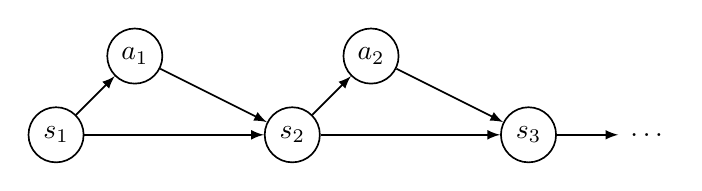
\begin{tikzpicture}[-latex ,auto ,node distance =1 cm and 1cm ,
      on grid , inner sep=0pt, minimum size=7mm,
      semithick, state/.style={circle, draw}]
      % s1, a1, s2;
      \node[state](s_1) at(0,0) {$s_1$};
      \node[state](a_1) at(1,1) {$a_1$};                                                                                                       
      \path (s_1) edge (a_1);
      \node[state](s_2) at(3,0) {$s_2$};
      \path (s_1) edge (s_2);
      \path (a_1) edge (s_2);
      % s2, a2, s3
      \node[state] (a_2) at(4,1) {$a_2$};
      \path (s_2) edge (a_2);
      \node[state] (s_3) at(6,0){$s_3$};
      \path (s_2) edge (s_3);
      \path (a_2) edge (s_3);
      % dots;
      \node (dots) at(7.5,0) {$\ldots$};
      \path (s_3) edge (dots);
  \end{tikzpicture}
  \caption{\label{fig:MDP} Graph of MDP with Markovian states.}
\end{figure}

As mentioned earlier with the robot example, we can have our agent 
not observe the Markovian state, and instead receive an observation, 
$o_t$, from its sensors. This observation is associated with 
an emission operator $\mathcal{E}$, that defines a (possibly stochastic) 
mapping from the state space, $\mathcal{S}$, to the observation 
space, $\mathcal{O}$. This induces a Partially Observed MDP (POMDP) 
whose graphical model is presented in Figure \ref{fig:POMDP}. The 
POMDP is defined by the tuple ($\mathcal{S}$, $\mathcal{A}$, 
$\mathcal{O}$, $\mathcal{P}$, $\mathcal{E}$, $r(\cdot)$, $\gamma$), 
where $\mathcal{O}$ and $\mathcal{E}$ are the observation space and 
the emission operator respectively and everything else in the tuple 
is the same as for the MDP case. It is important to note that the 
reward function is still dependent on the states, and not the observations 
since it specifies the goal and is external to the agent. Intuitively, 
the environment is oblivious to the sensory limitations of the agent 
and only bases its reward signal on the current configuration/state and 
the action that is selected by the agent.

As we 
can read off of the pgm in Figure \ref{fig:POMDP}, we see that given 
$s_t$ and $a_t$, $s_{t+1}$ is still independent of 
$o_{1:t}$, $s_{1:t-1}$ and $a_{1:t-1}$ by D-separation.
The observations, however, are not Markovian in general 
since $o_j$ for $j<t$ 
can influence $o_{t+1}$ even if $o_t$ and $a_t$ are known (again by 
D-separation).

\begin{figure}[H]
  \centering
  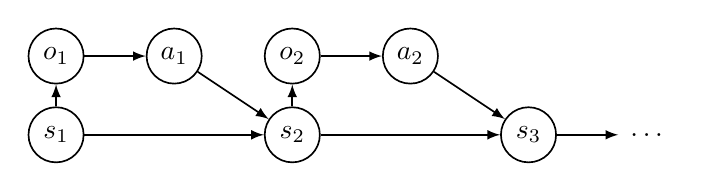
\begin{tikzpicture}[-latex ,auto ,node distance =1 cm and 1cm ,
      on grid , inner sep=0pt, minimum size=7mm,
      semithick, state/.style={circle, draw}]
      % s1, o1, a1, s2;
      \node[state](s_1) at(0,0) {$s_1$};
      \node[state](o_1) at (0, 1){$o_1$};
      \path (s_1) edge (o_1);
      \node[state](a_1) at(1.5,1) {$a_1$};
      \path (o_1) edge (a_1);
      \node[state](s_2) at(3,0) {$s_2$};
      \path (s_1) edge (s_2);
      \path (a_1) edge (s_2);
      % s2, o2, a2, s3
      \node[state](o_2) at (3,1) {$o_2$};
      \path (s_2) edge (o_2);
      \node[state] (a_2) at(4.5,1) {$a_2$};
      \path (o_2) edge (a_2);
      \node[state] (s_3) at(6,0){$s_3$};
      \path (s_2) edge (s_3);
      \path (a_2) edge (s_3);
      % dots;
      \node (dots) at(7.5,0) {$\ldots$};
      \path (s_3) edge (dots);
  \end{tikzpicture}
  \caption{\label{fig:POMDP} Graph of POMDP, $s_t$ is the Markovian 
  state, $o_t$ is the observation of the agent.}
\end{figure}

The associated factorisation based on the pgm in 
Figure \ref{fig:POMDP} is:
\begin{equation}
  p^{\pi}(\tau)=p(s_1)\prod_{t=1}^T p(o_t|s_t)\pi(a_t|o_t)p(s_{t+1}|s_t, a_t).
\end{equation}
We see that in the POMDP setting, the agent makes decisions based 
on the observation and not the Markovian state. Depending on how 
informative the observation is, it may be difficult to construct 
a well-performing policy. Additionally, due to the non-Markovian 
nature of the observations, it is common to track and process old 
observations in order to form the agent state. Intuitively, one 
would expect the influence of observations from a long time ago 
to decay, so it might be useful to have a moving window over the 
collected experience.

In cases where we have deterministic transitions from state and action 
to the next state (and similarly from state to observation), 
$p(s_{t+1}|s_t, a_t)=\delta(s_{t+1},f(s_t, a_t))$, where 
$\delta(\cdot)$ denotes the delta distribution (placing all 
probability mass on $f(s_t, a_t)$) and 
$f: \mathcal{S}\times\mathcal{A}\rightarrow \mathcal{S}$ is some deterministic 
transition function (similarly $g:\mathcal{S}\rightarrow \mathcal{O}$ 
can be the sensor mapping the state to the observation).

%%%%%%%%%%%%%%%%%%%%%%%%%%%%%%%%%%%%%%%%%%%%%%%%%
% SECTION - FORMULATING EPISODIC AND CONTINUAL SETTING REWARD;
\section{Formulating objective functions}\label{sec:RLGoalMaths}
In Section \ref{sec:RLGoal} we explained the goal of RL in words. 
In this section we will give a more formal mathematical definition. 
To that end we will first define the finite/episodic case objective, 
and then define the continual setting objective.

First, recall the Monte Carlo return Equation \ref{eq:MCReturn}. The episodic 
objective is to find a behaviour/policy, $\pi(\cdot)$, that maximises 
the expected Monte Carlo return over the distribution of finite 
trajectories, induced by the policy. 
This is summarised by Equation \ref{eq:ep_objective}.
\begin{align}
  \label{eq:ep_objective}
  \pi^*&=\arg \max_{\pi}\; \mathbb{E}_{\tau\sim p^{\pi}(\tau)}[G_0(\tau)]\notag\\
  &=\arg \max_{\pi}\; \mathbb{E}_{\tau\sim p^{\pi}(\tau)}\left[\sum_{t=1}^{\text{len}(\tau)}\gamma^{t-1}r(a_{t}, s_{t})\right].
\end{align}
In Equation \ref{eq:ep_objective}, $\text{len}(\tau)$ denotes the length of the episode.

Before we tackle the continual setting, observe that the MDP in 
Figure \ref{fig:MDP} can be seen as a Markov chain where we define 
the new state $z_t:=(s_t, a_t)$. Based on this formulation we also 
get a new transition operator 
$p(a_{t+1},s_{t+1}|a_t,s_t)=\pi(a_{t+1}|s_{t+1})p(s_{t+1}|a_t,s_t)$ and 
the corresponding pgm can be observed in Figure \ref{fig:MCz}.

\begin{figure}[H]
  \centering
  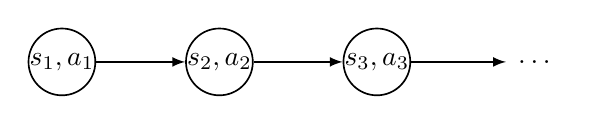
\begin{tikzpicture}[-latex ,auto ,node distance =1 cm and 1cm ,
      on grid , inner sep=0pt, minimum size=7mm,
      semithick, state/.style={circle, draw}]
      % s1, a1, s2;
      \node[state](z_1) at(0,0) {$s_1,a_1$};
      \node[state](z_2) at(2,0) {$s_2, a_2$};
      \path (z_1) edge (z_2);
      \node[state](z_3) at(4,0) {$s_3, a_3$};
      \path (z_2) edge (z_3);
      \node (dots) at(6,0) {$\ldots$};
      \path (z_3) edge (dots);
  \end{tikzpicture}
  \caption{\label{fig:MCz} Markov chain induced by MDP.}
\end{figure}

It can be shown that if the Markov chain is aperiodic and if there 
is a path to all possible tuples $(s_t, a_t)$ from any other tuple 
$(s_j, a_j)$, then an equilibrium distribution exists, which 
tells us the long-term probability of visiting a state-action tuple 
$\mu(s_t, a_t)$.

Observe that we could also rewrite the episodic definition as:
\begin{align}
  \label{eq:cont_objective}
  \pi^*&=\arg \max_{\pi}\; \mathbb{E}_{\tau\sim p^{\pi}(\tau)}[G_0(\tau)]\notag\\
  &=\arg \max_{\pi}\; \mathbb{E}_{\tau\sim p^{\pi}(\tau)}\left[\sum_{t=1}^{\text{len}(\tau)}\gamma^{t-1}r(a_{t}, s_{t})\right]\notag\\
  &=\arg \max_{\pi}\; \sum_{t=1}^{\text{maxlen}(\tau)}\mathbb{E}_{s_{t}, a_{t}\sim p^{\pi}(s_{t}, a_{t})}[r(s_t, a_t)\gamma^{t-1}]\notag\\
  &=\arg \max_{\pi}\; \frac{1}{\text{maxlen}(\tau)}\sum_{t=1}^{\text{maxlen}(\tau)}\mathbb{E}_{s_{t}, a_{t}\sim p^{\pi}(s_{t}, a_{t})}[r(s_{t}, a_{t})\gamma^{t-1}],
\end{align}
where $\text{maxlen}(\tau)$ is the maximum length of a trajectory possible under $\pi$. 
In the continual setting, $\text{maxlen}(\tau)\rightarrow\infty$, and provided the 
equilibrium distribution for the Markov Chain in Figure 
\ref{fig:MCz} exists, 
after some time (burn-in), $p^{\pi}\rightarrow \mu^{\pi}$. Intuitively,
 due to the division by $\text{maxlen}(\tau)$, 
the first finite number of steps from $p^{\pi}$ 
will be negligable and only the steps sampled according to the equilibrium, 
$\mu^{\pi}$ will persist. This intuition, helps us arrive at the 
continual objective known as expected long-term reward:
\begin{equation}\label{eq:continualObjective}
  \arg \max_{\pi}\; {E}_{s, a\sim \mu^{\pi}(s, a)}[r(s, a)],
\end{equation}
where $\mu^{\pi}$ is the limiting distribution of the Markov chain 
induced by $\pi$ as seen in Figure \ref{fig:MCz}.



%%%%%%%%%%%%%%%%%%%%%%%%%%%%%%%%%%%%%%%%%%%%%%%%%%%%%%%%%%
% NEW SECTION - VALUE FUNCS;
\section{Value functions}\label{sec:valueFuncs}
A key quantity in our application and of much of modern Reinforcement Learning 
are the value functions. These quantities aim to estimate the 
expected future return, given the current state or state-action pair. 
We shall derive those quantities from the RL objective functions 
defined in the previous section.

Starting from the episodic objective Equation \ref{eq:ep_objective},
\begin{align}\label{eq:valFuncDef}
  \mathbb{E}_{\tau\sim p^{\pi}(\tau)}\left[\sum_{t=1}^{\text{len}(\tau)}r(s_t, a_t)\gamma^{t-1}\right]
  &=\mathbb{E}_{s_1\sim p(s_1)}\left[\mathbb{E}_{\tau\sim p^{\pi}(\tau|s_1)}\left[\sum_{t=1}^{\text{len}(\tau)}r(s_t, a_t)\gamma^{t-1}|s_1\right]\right]\notag\\
  &=\mathbb{E}_{s_1\sim p(s_1)}\left[
      \mathbb{E}_{a_1\sim \pi(\cdot|s_1)}\left[
          r(s_1, a_1) + 
          \mathbb{E}_{\tau\sim p^{\pi}(\tau|s_1,a_1)}\left[\sum_{t=2}^{\text{len}(\tau)}r(s_t, a_t)\gamma^{t-1}\right]|s_1,a_1
        \right]
    \right]\notag\\
  &=:\mathbb{E}_{s_1\sim p(s_1)}\left[
      \mathbb{E}_{a_1\sim \pi(\cdot|s_1)}\left[Q^{\pi}(s_1,a_1)\right]
      \right]\notag\\
      &=:\mathbb{E}_{s_1\sim p(s_1)}\left[
        V^{\pi}(s_1)
      \right],
\end{align}
where $Q^{\pi}(s_1,a_1):=\mathbb{E}[G_0(\tau)|s_1, a_1, \pi]$ is the state-action value function,  
sometimes referred to as the Q-function, and $V^{\pi}:=\mathbb{E}_{a_1\sim\pi(\cdot)}[Q^{\pi}(s_1, a_1)|s_1]$ is the state-value 
function.

In Equation \ref{eq:valFuncDef} we already used a form of the Bellman expectation/prediction 
equation:
\begin{align}\label{eq:bellmanv}
  V^{\pi}(s)&=\mathbb{E}_{a\sim \pi(\cdot|s)}[Q^{\pi}(s, a)|s]\notag\\
  &=\mathbb{E}_{a\sim \pi(\cdot|s)}\left[r(s, a) + \gamma \sum_{s'\in \mathcal{S}}p(s'|s,a)V^{\pi}(s')|s\right].
\end{align}

The same for the Q-function is given by Equation \ref{eq:bellmanq}.
\begin{align}\label{eq:bellmanq}
  Q^{\pi}(s, a)&=r(s, a) + \gamma \sum_{s'\in \mathcal{S}}p(s'|s, a)V^{\pi}(s')\notag\\
  &= r(s,a) + \gamma \sum_{s'\in \mathcal{S}}p(s'|s, a)\sum_{a'\in \mathcal{A}}\pi(a'|s')Q^{\pi}(s', a').
\end{align}

The other pair of Bellman equations are known as the Bellman optimality 
equations and enforce a consistency criterion for optimal policies. 
\begin{align}\label{eq:bellmanOptV}
  V^{\pi^*}(s)&=\max_{a\in \mathcal{A}}\; \left[r(s, a) + \gamma \sum_{s'\in \mathcal{S}}p(s'|s,a)V^{\pi}(s')|s\right]\notag\\
  &=\max_{a\in \mathcal{A}}\;Q^{\pi^*}(s, a).
\end{align}

\begin{align}\label{eq:bellmanOptQ}
  Q^{\pi^*}(s,a)&=r(s,a) + \gamma \sum_{s'\in \mathcal{S}}p(s'|s, a)\max_{a'\in \mathcal{A}}\;Q^{\pi*}(s', a').
\end{align}

It can be shown that there always exists at least one optimal 
policy \citep{Sutton1998}, and the Bellman optimality Equations 
in \ref{eq:bellmanOptV} and \ref{eq:bellmanOptQ} can be viewed 
as consistency equations for an optimal policy $\pi^*$.

%%%%%%%%%%%%%%%%%%%%%%%%%%%%%%%%%%%%%%%%%%%%%%%%%%%%%%%%%%%
% SECTION - improving the policy;
\section{Value iteration}\label{sec:ValueIter}
Based on the Value functions, $Q^{\pi}$ and $V^{\pi}$ introduced in the 
previous section, there exists a powerful paradigm that allows 
us to arrive at an optimal policy. This paradim is called Generalised 
Policy Iteration.

Given a policy one might be interested in understanding how good 
it is - evalueate it. Another question, given a current policy, 
might be whether we can improve it. In the tabular case, where 
we can enumarate all state-action pairs, it can be shown that 
for $\gamma\in[0, 1)$, the updates given in Equation 
\ref{eq:policyEval} correspond to operators 
leading to a convergent sequence, whose stationary point is the 
value of the policy $\pi$.
\begin{align}\label{eq:policyEval}
  v_{k+1}(s_t) &\gets \mathbb{E}[r_{t+1} + \gamma v_k(s_{t+1})|s_t]\notag\\
  q_{k+1}(s_t, a_t)&\gets r(s_t, a_t) 
  + \gamma\mathbb{E}[q_{k}(s_{t+1}, a_{t+1})|s_t,a_t].
\end{align}

We can iterate the Equations in \ref{eq:policyEval} until $v_{k+1}(s)=v_k(s)$ 
$\forall s\in \mathcal{S}$ at which point we get $v_k\approx v^{\pi}$ 
(and similarly for $q$).


For the policy improvement step, it can be shown \citep{Sutton1998} 
that after the 
policy evaluation converges, updating the policy 
to be greedy with respect to the action value $q^{\pi}$ of the 
current policy, improves the policy.
\begin{equation}\label{eq:policyImp}
  \pi'(s)=\arg \max_a q^{\pi}(s, a).
\end{equation}

Together, the Equations for policy evaluation \ref{eq:policyEval} 
and policy improvement \ref{eq:policyImp} 
can be iterated one after another until we reach an optimal policy 
given an MDP.

It is worth noting, that instead of waiting for policy evaluation 
to converge, we can instead do just one sweep 
of updates (single iteration) and then immediately do a policy 
improvement step. This procedure is known as value iteration and 
can also be shown to converge to the value functions of an 
optimal policy given an MDP. The equations for value iteration 
are shown in \ref{eq:valueIter}
\begin{align}\label{eq:valueIter}
  v_{k+1}(s_t)&\gets\max_a \left[r(s_t, a) 
  + \gamma \sum_{s'\in\mathcal{S}}p(s'|s_t, a)v_{k}(s')\right]\notag\\
  q_{k+1}(s_t, a_t)&\gets r(s_t, a_t) 
  + \gamma \sum_{s'\in\mathcal{S}}p(s'|s_t, a_t)\max_a\; q_{k}(s', a).
\end{align}


%%%%%%%%%%%%%%%%%%%%%%%%%%%
% NEW SECTION - Q-learning;
\section{Q-learning}\label{sec:Qlearning}
In this section we use Q-learning \citep{QlearningWatkins1992} 
as a motivating example 
for single-step off-policy methods. These are methods 
that aim to evaluate a target policy, $\pi$, while following 
a different behaviour policy, $\mu$.

The simplest way to understand Q-learning, is perhaps by 
first introducing an on-policy variant called SARSA \citep{SARSA}. 
SARSA is an algorithm that samples the policy evaluation update 
for the Q-function as given in Equation \ref{eq:policyEval}.
The sampling is done based on the current policy/behaviour and can 
be motivated by stochastic gradient descent on the Squared Error of 
the true Q-function, $Q^{\pi}$, and our current estimate $Q_{k}$.
Intuitively, taking a gradient with respect to $Q_{k}$ we get the 
expression in Equation \ref{eq:sarsaGrad}.
\begin{align}\label{eq:sarsaGrad}
  \frac{\partial}{\partial Q_{k}}(Q^{\pi}(s_t, a_t) - Q_{k}(s_t, a_t))^2&=-2(Q^{\pi}(s_t, a_t) - Q_{k}(s_t,a_t)).
\end{align}

Since we do not know the true $Q^{\pi}$ (otherwise we would be done) 
we receive a reward, $r_{t+1}$, and the next state $s_{t+1}$ 
based on taking action $a_t$ at state $s_t$, then sample the next 
action, $a_{t+1}$, according to the current policy and instead of the 
true Q-function, we use our estimate $Q_{k}(s_{t+1}, a_{t+1})$ to evaluate 
the next state-action pair. This process gives the update in 
Equation \ref{eq:sarsa}.
The technique for using $Q_{k}(s_{t+1}, a_{t+1})$ instead 
of $Q^{\pi}(s_{t+1}, a_{t+1})$ is known as bootstrapping and needs to be 
handled with care since we may (usually are) following 
the direction of a biased gradient estimate. 
To this end, take note of the learning rate, $\alpha$ in Equation 
\ref{eq:sarsa} which is there to account for the noise introduced 
by bootstrapping.

Note that we did not require access to the model, $\mathcal{P}$, at 
any point. Because of this, SARSA is classified as a model-free method.

\begin{equation}\label{eq:sarsa}
  Q_{k+1}(s_t, a_t) = Q_{k}(s_t, a_t) + \alpha (r_{t+1} + \gamma Q_{k}(s_{t+1}, a_{t+1}) - Q_{k}(s_t, a_t)).
\end{equation}

% In Equation \ref{eq:sarsa}, first we interact with the environment 
% by proposing $a_t$, sampled by the current policy, then the environment 
% gives us the reward $r$ as feedback and transitions to the next state 
% $s_{t+1}$. At this point we once again sample an action $a_{t+1}$ 
% from the current policy and update in a gradient descent on the 
% Q-value fashion, towards the reward plus the discounted Q-value for 
% the next state action pair, $(s_{t+1},\; a_{t+1})$.

While SARSA evaluates the current policy $\pi$, Q-learning aims 
to evaluate the greedy policy given the current estimate $Q_{k}$, 
while following another policy, $\mu$, known as the behaviour. 
This is why Q-learning is an off-policy method.

The associated update (for tabular Q-learning) is given in Equation 
\ref{eq:qlearning}
\begin{equation}\label{eq:qlearning}
  Q_{k+1}(s_t, a_t) = Q_{k}(s_t, a_t) + \alpha \left(r_{t+1} + \gamma \max_{a'\in\mathcal{A}}\;Q_{k}(s_{t+1}, a') - Q_{k}(s_t, a_t)\right).
\end{equation}

The reader may have noticed that the update for Q-learning is like 
a sampled version of the value iteration Equation \ref{eq:valueIter} 
for the Q-function. Both SARSA and Q-learning can be shown to 
converge given appropriately decaying learning rates $\alpha$ 
that satisfy the Robbins-Monro conditions given in Equation 
\ref{eq:RobbinsMonro} and a behaviour, $\mu$, that explores 
sufficiently often (needed for Q-learning).

\begin{align}\label{eq:RobbinsMonro}
  \sum_{k=0}^\infty \alpha_k&\rightarrow \infty\notag\\
  \sum_{k=0}^\infty \alpha_k^2&< \infty.
\end{align}

%%%%%%%%%%%%%%%%%%%%%%%%%%%%%%%%%%%%%%%5
% NEW SECTION;
\section{Policy Gradients}\label{sec:PolicyGrads}
In the previous sections we have focused on ways to estimate 
value functions, which we can then use to derive a policy implicitly. 

In this section we introduce methods from 
the policy-based RL family, where we explicitly 
parameterise a policy function 
$\pi_\theta$ and aim to estimate its parameters. This is perhaps 
the most direct-looking way to achieve the goal of RL as defined 
in Section \ref{sec:RLGoal}.

Before we begin, it is worth inspecting the pgm of the MDP
in Figure \ref{fig:MDPRew}, 
this time having included the rewards. Note how the reward 
at time $t$ does not depend on future actions and/or states 
given the state and action at time $t-1$.
\begin{figure}[H]
  \centering
  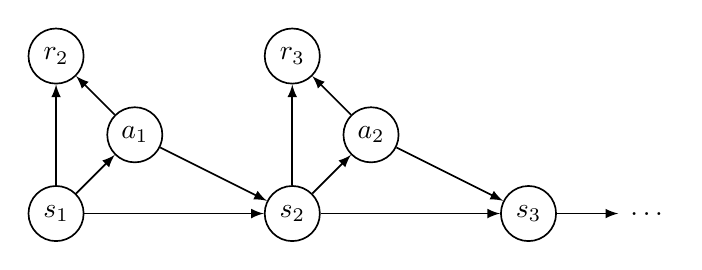
\begin{tikzpicture}[-latex ,auto ,node distance =1 cm and 1cm ,
      on grid , inner sep=0pt, minimum size=7mm,
      semithick, state/.style={circle, draw}]
      % s1, a1, s2;
      \node[state](s_1) at(0,0) {$s_1$};
      \node[state](a_1) at(1,1) {$a_1$};                                                                                                       
      \path (s_1) edge (a_1);
      \node[state](r_2) at(0, 2) {$r_2$};
      \node[state](s_2) at(3,0) {$s_2$};
      \path (s_1) edge (s_2);
      \path (a_1) edge (s_2);
      \path (s_1) edge (r_2);
      \path (a_1) edge (r_2);
      % s2, a2, s3
      \node[state] (a_2) at(4,1) {$a_2$};
      \path (s_2) edge (a_2);
      \node[state] (r_3) at(3, 2) {$r_3$};
      \node[state] (s_3) at(6,0){$s_3$};
      \path (s_2) edge (s_3);
      \path (a_2) edge (s_3);
      \path (s_2) edge (r_3);
      \path (a_2) edge (r_3);
      % dots;
      \node (dots) at(7.5,0) {$\ldots$};
      \path (s_3) edge (dots);
  \end{tikzpicture}
  \caption{\label{fig:MDPRew} Graph of MDP including rewards.}
\end{figure}

We derive Policy Gradients \citep{REINFORCE} 
by starting from the episodic objective as introduced in Section 
\ref{sec:RLGoalMaths}. Due to parameterising our policy 
with parameters, $\theta$, and assuming it is among a 
class of functions who are 
differentiable in $\theta$, we reformulate the episodic 
objective as given in Equation \ref{eq:PGObjective}.

\begin{align}\label{eq:PGObjective}
  J_\theta&:=\mathbb{E}_{\tau\sim p_{\theta}(\tau)}
   \left[
    \sum_{t=1}^{\text{len}(\tau)}\gamma^{t-1}r(a_t, s_t)\right]\notag\\ 
  \theta^*&=\arg \max_{\theta}J_\theta.
\end{align}

The gradient of this objective with respect to the parameters, $\theta$ 
of the policy is derived in Equation \ref{eq:PGDerive}.
\begin{align}\label{eq:PGDerive}
  \nabla J_\theta&=\nabla\sum_{\tau}p_{\theta}(\tau)\sum_{t=1}^{\text{len}(\tau)}\gamma^{t-1}r(s_t, a_t)\notag\\
  &=\sum_{\tau}\nabla p_{\theta}(\tau)\sum_{t=1}^{\text{len}(\tau)}\gamma^{t-1}r(s_t, a_t)\notag\\
  &=\sum_{\tau}p_{\theta}(\tau)\nabla \log p_\theta(\tau)\sum_{t=1}^{\text{len}(\tau)}\gamma^{t-1}r(s_t, a_t)\notag\\
  &=\sum_{\tau}p_{\theta}(\tau)\left(
    \sum_{t=1}^{\text{len}(\tau)}\nabla \log \pi_\theta(a_t|s_t)
  \right)\sum_{k=1}^{\text{len}(\tau)}\gamma^{k-1}r(s_k, a_k)\notag\\
  &=\sum_{\tau}p_\theta(\tau)\sum_{t=1}^{\text{len}(\tau)}\nabla \log \pi_\theta(a_t|s_t)
  \left(
    \sum_{k=1}^{t-1}\gamma^{k-1}r(s_k, a_k)
    + \sum_{k=t}^{\text{len}(\tau)}\gamma^{k-1}r(s_k, a_k)
  \right)\notag\\
  &=\sum_{\tau}p_\theta(\tau)\sum_{t=1}^{\text{len}(\tau)}\nabla \log \pi_\theta(a_t|s_t)
  \left(
    \sum_{k=t}^{\text{len}(\tau)}\gamma^{k-1}r(s_k, a_k)
  \right)\notag\\
  &=\sum_{\tau}p_\theta(\tau)\sum_{t=1}^{\text{len}(\tau)}\nabla \log \pi_\theta(a_t|s_t)
  \gamma^{t-1}\left(
    \sum_{k=t}^{\text{len}(\tau)}\gamma^{k-t}r(s_k, a_k)
  \right)\notag\\
  &=\sum_{\tau}p_\theta(\tau)\sum_{t=1}^{\text{len}(\tau)}\nabla \log \pi_\theta(a_t|s_t)
  \gamma^{t-1}G_t(\tau_{t:})\notag\\
  &=\mathbb{E}_{\tau\sim p_\theta(\tau)}\left[\sum_{t=1}^{\text{len}(\tau)}\nabla \log \pi_\theta(a_t|s_t)
  \gamma^{t-1}G_t(\tau_{t:})\right]\notag\\
  &=\mathbb{E}_{\tau\sim p_\theta(\tau)}\left[\sum_{t=1}^{\text{len}(\tau)}\nabla \log \pi_\theta(a_t|s_t)
  \gamma^{t-1}Q^{\pi}(s_t, a_t)\right].
\end{align}

While deriving Equation \ref{eq:PGDerive} we have used the 
fact in Equation \ref{eq:dropPrevRews}.

\begin{align}\label{eq:dropPrevRews}
  \sum_{\tau}p_\theta(\tau)\nabla \log \pi_\theta(a_t|s_t)
  \left(
    \sum_{k=1}^{t-1}\gamma^{k-1}r(s_k, a_k)
  \right)\notag\\
  &=\sum_{\tau_{:t}}p_\theta(\tau_{:t})\left(
    \sum_{k=1}^{t-1}\gamma^{k-1}r(s_k, a_k)
  \right)\sum_{a_t\in\mathcal{A}}\pi_\theta(a_t|s_t)
  \nabla \log \pi(a_t|s_t)\sum_{\tau_{t+1:}}p_\theta(\tau_{t+1:})\notag\\
  &=\sum_{\tau_{:t}}p_\theta(\tau_{:t})\left(
    \sum_{k=1}^{t-1}\gamma^{k-1}r(s_k, a_k)
  \right)\sum_{a_t\in\mathcal{A}}\pi_\theta(a_t|s_t)
  \nabla \log \pi(a_t|s_t)\notag\\
  &=\sum_{\tau_{:t}}p_\theta(\tau_{:t})\left(
    \sum_{k=1}^{t-1}\gamma^{k-1}r(s_k, a_k)
  \right)\sum_{a_t\in\mathcal{A}}\pi_\theta(a_t|s_t)\frac{\nabla\pi(a_t|s_t)}{\pi_\theta(a_t|s_t)}\notag\\
  &=\sum_{\tau_{:t}}p_\theta(\tau_{:t})\left(
    \sum_{k=1}^{t-1}\gamma^{k-1}r(s_k, a_k)
  \right)\nabla\sum_{a_t\in\mathcal{A}}\pi_\theta(a_t|s_t)\notag\\
  &=\sum_{\tau_{:t}}p_\theta(\tau_{:t})\left(
    \sum_{k=1}^{t-1}\gamma^{k-1}r(s_k, a_k)
  \right)\times 0\notag\\
  &=0.
\end{align}

Where in the above we used the short-hand notation:
\begin{align*}
  \sum_{\tau_{:t}}p_\theta(\tau_{:t})&=\sum_{s_1,a_1,\ldots,s_t}p(s_1)\prod_{k=1}^{t-1}\pi_\theta(a_k|s_k)p(s_{k+1}|s_k,a_k),\notag\\
  \sum_{\tau_{t+1:}}p_\theta(\tau_{t+1:})&=\sum_{s_{t+1}, a_{t+1},\ldots,s_{\text{len}(\tau)}}p(s_{t+1}|s_t,a_t)\prod_{k=t+1}^{\text{len}(\tau)-1}\pi(a_k|s_k)p(s_{k+1}|s_k,a_k).
\end{align*}

Taking a closer look at Equation \ref{eq:PGDerive}, we see that 
if we sample it, we get Equation \ref{eq:sampledPG}.
\begin{equation}\label{eq:sampledPG}
  \sum_{n=1}^N
    \sum_{t=1}^{\text{len}(\tau^{(n)})}\nabla \log \pi_\theta(a_t^{(n)}|s_t^{(n)})
  \gamma^{t-1}G_t(\tau_{t:}^{(n)}).
\end{equation}

This is very similar to maximum likelihood estimation of $\theta$ 
given trajectories sampled according to $p_\theta$, however, 
also weighted by a discounted return $\gamma^{t-1}G_t(\tau_{t:}^{(n)})$.
Intuitively, we wish to maximise the likelihood of trajectories 
that resulted in greater returns.

\section{Actor-Critics}\label{sec:ActorCritic}
In Section \ref{sec:PolicyGrads} we derived the policy gradient 
update rule and gave an intuitive relation to maximum likelihood 
where we wish to increase the likelihood of episodes resulting 
in greater returns. This makes the policy gradients dependent of 
the form of the returns. Suppose the high returns are zeros and 
the low returns are negative. If the high returns are zeros, then 
the update associated with them will vanish. This makes the policy 
gradients dependent on the type of reward function of the environment 
and can cause policy gradients to be very noisy in finite samples.

Actor Critics \citep{Tsitsiklis} are a way to aleviate this issue 
by introducing a baseline function, to which the returns are compared.
Returns who score higher than the baseline are associated with 
beneficial behaviour and we wish to increase the likelihood 
of actions leading to such behaviour/returns.

To make this concrete, consider the baseline $b(s_t)$, that depends 
on $s_t$.

\begin{theorem}\label{thm:baselineThm}
  \begin{equation*}
    \mathbb{E}_{\tau\sim p_\theta(\tau)}\left[\nabla \log \pi_\theta(a_t|s_t)
    b(s_t)\right]=0.  
  \end{equation*}
\end{theorem}

\begin{proof}
  \begin{align}
    \mathbb{E}_{\tau\sim p_\theta(\tau)}\left[\nabla \log \pi_\theta(a_t|s_t)
    b(s_t)\right]&= \sum_{\tau}p_\theta(\tau)\nabla \log\pi_\theta(a_t|s_t)b(s_t)\notag\\
    &=\sum_{\tau_{:t}}p_\theta(\tau_{:t})b(s_t)\sum_{a_t\in\mathcal{A}}\pi_\theta(a_t|s_t)\nabla \log\pi_\theta(a_t|s_t) \sum_{\tau_{t+1:}}p_\theta(\tau_{t+1:})\notag\\
    &=\sum_{\tau_{:t}}p_\theta(\tau_{:t})b(s_t)\sum_{a_t\in\mathcal{A}}\pi_\theta(a_t|s_t)\nabla \log\pi_\theta(a_t|s_t)\notag\\
    &=\sum_{\tau_{:t}}p_\theta(\tau_{:t})b(s_t)\times 0\notag\\
    &=0,
  \end{align}
  where, similarly to in the policy gradient derivation, we used the fact that 
  \begin{equation*}
    \sum_{a_t\in\mathcal{A}}\pi_\theta(a_t|s_t)\nabla \log\pi_\theta(a_t|s_t)=0. 
  \end{equation*}
\end{proof}

Based on Theorem \ref{thm:baselineThm} we have that:
\begin{theorem}\label{thm:unbiasedBaseline}
  Given a baseline, $b(s_t)$, that does not depend on the actions,\\
  $\mathbb{E}_{\tau\sim p_\theta(\tau)}\left[\sum_{t=1}^{\text{len}(\tau)}\nabla \log \pi_\theta(a_t|s_t)
  \gamma^{t-1}\left(Q^{\pi}(s_t, a_t)-b(s_t)\right)\right]$ is unbiased with respect 
  to the policy gradient update in Equation \ref{eq:PGDerive}.
\end{theorem}
Due to Theorem \ref{thm:baselineThm}, we can pick any function 
$b(\cdot)$ that does not depend on the actions as a baseline and 
get an unbiased policy gradient update. In the case of Actor-Critics, 
$b(s_t)=V^{\pi}(s_t)$, or an approximation thereof, $V_{\phi}$.

The Actor-Critic update is then given in Equation \ref{eq:ActorCritic}.
\begin{equation}\label{eq:ActorCritic}
  \mathbb{E}_{\tau\sim p_\theta(\tau)}\left[\sum_{t=1}^{\text{len}(\tau)}\nabla \log \pi_\theta(a_t|s_t)
  \gamma^{t-1}\left(Q^{\pi}(s_t, a_t)-V^{\pi}(s_t)\right)\right].
\end{equation}

The term $Q^{\pi}(s_t,a_t)-V^{\pi}(s_t)$ is sometimes called the 
advantage due to taking action $a_t$ at state $s_t$. This is 
due to the Bellman Expectation equation for the state-value function 
as given in Equation \ref{eq:bellmanv}. Since $V^{\pi}$ is the 
expected Q-function, integrating over the actions, there are 
actions for which the Q-function is greater than or equal to the 
state-value function. Such actions are advantageous, since they are 
likely to lead us to trajectories that yield high returns (since the 
Q-function is itself the expected future return given start at 
the relevant state and action). The Actor-Critic aims to 
increase the likelihood of advantageous actions, therefore.

In practice, $V^{\pi}$ is approximated by e.g., a parameterised 
state-value function $V_\phi$, which is learned by some policy 
evaluation method. Such methods can be as simple as just 
substituting the Q-function for the state-value function 
in the Equation for SARSA \ref{eq:sarsa}, which results in 
a method called TD(0) \citep{SuttonTD}. 
The Q-function, $Q^{\pi}$ is often also approximated 
either by the relevant Monte Carlo return as given in Equation 
\ref{eq:MCReturn} or by bootstrapping as in the 
case of SARSA.


%%%%%%%%%%%%%%%%%%%%%%%%%%%%%%%%%%%%%%%%%%%%%%%%%%%%%%5
% NEW CHAPTER - MaxEntRL
\chapter{Maximum Entropy Reinforcement Learning}\label{chap:MaxEntRL}
Maximum Entropy Reinforcement Learning (MaxEntRL) is most commonly 
motivated by observing the behaviour of biological systems, assuming 
they are rational agents and that they act the way they do in order to achieve 
a certain goal. The crucial point here is that although all 
demonstrations are assumed to achieve the goal of the agent, 
they are allowed to deviate from one-another in ways that 
do not impact their successful outcome. That being said, 
some demonstrations may be more desirable than others, e.g., 
because they make fewer unnecessary steps to achieve the goal.

This definition makes 
traditional optimal control theory inappropriate for modelling 
this behaviour and understanding why we observed the different 
paths. This is because, it can be shown that under the objective 
introduced in Section \ref{sec:RLGoalMaths}, given full observability 
(Markov states), there exists an optimal policy that 
is deterministic \citep{Sutton1998}.
This cannot help us explain the variability in the agent's demonstrations,
therefore.

In order to be able to learn a good behaviour, we still 
need to somehow differentiate between demonstrations and tell 
which ones are more desirable to emulate. 
In his paper \cite{Ziebart2008} aims to create an ordering among 
observed demonstrations by weighting the trajectories 
by the exponential of the sum of rewards (the return) along 
the given trajectory. In this way, demonstrations with greater 
returns 
will be exponentialy more desirable than others. A simple illustration 
of the soft-optimal control (SOC) idea is portrayed in Figure \ref{fig:softopt}. 
In this figure, we see the optimal control behaviour, and the 
soft-optimal demonstrations alongside it.


\begin{figure}[H]
  \begin{center}
    \includegraphics[scale=0.5]{optControlVsSoftOpt.png}
  \end{center}
  \caption{\label{fig:softopt}Simple illustration of Optimal 
  Control vs Soft Optimal 
  Control. The blue solid line represents the deterministic optimal 
  control to reach from the red ``X'' on the left to the 
  red ``X'' on the right. The remaining lines 
  are noisy perturbations of the intermediate points 
  between the starting and ending ``X'' - demonstrating 
  soft optimality.}
\end{figure}


%%%%%%%%%%%%%%%%%%%%%%%%%%%%%%%%%%%%%%%%%%%%%%%%%%%%%%%%%%%%
% NEW SECTION - SOC;
\section{Soft Optimal Control}\label{sec:SOC}

A very illustrative way to understand soft-optimal control (SOC) 
is provided in \cite{LevineRLasInf}, where the associated 
pgm is a Directed Acyclic Graph (DAG) such as the one 
seen in Figure \ref{fig:SOCGraph}.

\begin{figure}[H]
  \centering
  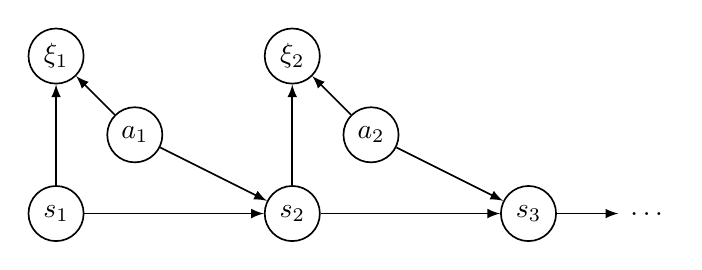
\begin{tikzpicture}[-latex ,auto ,node distance =1 cm and 1cm ,
      on grid , inner sep=0pt, minimum size=7mm,
      semithick, state/.style={circle, draw}]
      % s1, a1, s2;
      \node[state](s_1) at(0,0) {$s_1$};
      \node[state](a_1) at(1,1) {$a_1$};                                                                                                       
      % \path (s_1) edge (a_1);
      \node[state](xi_1) at(0, 2) {$\xi_1$};
      \node[state](s_2) at(3,0) {$s_2$};
      \path (s_1) edge (s_2);
      \path (a_1) edge (s_2);
      \path (s_1) edge (xi_1);
      \path (a_1) edge (xi_1);
      % s2, a2, s3
      \node[state] (a_2) at(4,1) {$a_2$};
      % \path (s_2) edge (a_2);
      \node[state] (xi_2) at(3, 2) {$\xi_2$};
      \node[state] (s_3) at(6,0){$s_3$};
      \path (s_2) edge (s_3);
      \path (a_2) edge (s_3);
      \path (s_2) edge (xi_2);
      \path (a_2) edge (xi_2);
      % dots;
      \node (dots) at(7.5,0) {$\ldots$};
      \path (s_3) edge (dots);
  \end{tikzpicture}
  \caption{\label{fig:SOCGraph} Graph of Soft-Optimal model. 
  The $\xi$ variables are binary optimality variables, equal to 
  $1$ with probability equal to $\exp(r(s_t, a_t))$.}
\end{figure}

Outside of the usual RL variables - states and actions - here, 
we also have binary ``optimality'' variables, $\xi_t\sim \text{Ber}(\exp(r(s_t, a_t)))$.
Where $\text{Ber}(\cdot)$ denotes the Bernoulli distribution. 
This means that we require the reward to be non-positive, which 
is easily achieved (in the case of bounded rewards) by subtracting 
the maximum reward.

It is worth noting that 
in \cite{Ziebart2008}, the graph is a Markov Random Field (MRF) 
where the states and actions share a potential function given 
by $\exp(r(s_t, a_t))$. This allows
the rewards to be positive.

We have chosen the formulation in \cite{LevineRLasInf} 
since it allows us to more 
easily convey the motivations behind SOC. In this exposition 
we explicitly define binary optimality variables at each step 
who we assume equalled $1$, for all demonstrated trajectories, 
signifying the optimality of these trajectories.

Based on the model defined by the pgm in Figure \ref{fig:SOCGraph}, 
we wish to estimate the policy of the agent, $p(a_t|s_t, \xi_{1:T}=1)$, 
assuming $\xi_t=1\;\forall t$, 
i.e., that the demonstrations are ``softly'' optimal. 
To this end, we employ the technique of message passing, and perform 
computations very similar to the ones performed in Hidden Markov Models 
(HHM).

Before we proceed with the derivations,
we first define short-hand notation in Equation \ref{eq:messages}, 
where $\beta$ are backward messages and $\alpha$ are forward messages.
\begin{align}\label{eq:messages}
  \beta_t(s_t, a_t)&:=p(\xi_{t:T}=1|s_t, a_t)\notag\\
  \beta_t(s_t)&:=p(\xi_{t:T}=1|s_t)\notag\\
  \alpha_t(s_t)&:=p(s_t, \xi_{1:t-1}=1).
\end{align}

The derivation of the message passing procedure can be seen 
in Equations \ref{eq:SOCQmessage}, \ref{eq:SOCVmessage} and 
\ref{eq:SOCforwardMessage}. Note that for brevity, we will use 
$\xi_{t:T}$ to mean $\xi_{t:T}=1$, i.e., that all optimality variables 
are equal to one.

\begin{align}\label{eq:SOCQmessage}
  \beta_t(s_t, a_t)&:=p(\xi_{t:T}=1|s_t, a_t)\notag\\
  &=p(\xi_t|s_t, a_t)p(\xi_{t+1:T}|s_t, a_t)\notag\\
  &=p(\xi_t|s_t, a_t)\int_{\mathcal{S}}p(\xi_{t+1:T}, s_{t+1}|s_t,a_t)ds_{t+1}\notag\\
  &=p(\xi_t|s_t, a_t)\int_{\mathcal{S}}p(\xi_{t+1:T}|s_{t+1})p(s_{t+1}|s_t,a_t)ds_{t+1}\notag\\
  &=p(\xi_t|s_t, a_t)\mathbb{E}_{s_{t+1}\sim p(s_{t+1}|s_t, a_t)}[\beta_t(s_{t+1})]\notag\\
  &=\exp(r(s_t, a_t))\mathbb{E}_{s_{t+1}\sim p(s_{t+1}|s_t, a_t)}[\beta_t(s_{t+1})].
\end{align}

\begin{align}\label{eq:SOCVmessage}
  \beta_t(s_t)&:=p(\xi_{t:T}|s_t)\notag\\
  &=\int_{\mathcal{A}}p(\xi_{t:T},a_t|s_t)da_t\notag\\
  &=\int_{\mathcal{A}}p(\xi_{t:T}|a_t, s_t)p(a_t|s_t)\notag\\
  &=\mathbb{E}_{a_t\sim p(a_t|s_t)}[\beta_t(s_t, a_t)].
\end{align}

\begin{align}\label{eq:SOCforwardMessage}
  \alpha_t(s_t)&:=p(s_t, \xi_{1:t-1}=1)\notag\\
  &=\int_{\mathcal{S}}\int_{\mathcal{A}}p(s_t, s_{t-1},a_{t-1},\xi_{1:t-1})da_{t-1}ds_{t-1}\notag\\
  &=\int_{\mathcal{S}}\int_{\mathcal{A}}p(s_t|s_{t-1}a_{t-1})p(\xi_{t-1}|s_{t-1},a_{t-1})p(a_{t-1}|s_{t-1})p(s_{t-1}, \xi_{1:t-2})da_{t-1}ds_{t-1}\notag\\
  &=\int_{\mathcal{S}}\int_{\mathcal{A}}p(s_t|s_{t-1}a_{t-1})p(\xi_{t-1}|s_{t-1},a_{t-1})p(a_{t-1}|s_{t-1})\alpha_{t-1}(s_{t-1})da_{t-1}ds_{t-1}.
\end{align}

In the above, $p(a_t|s_t)$ is not to be confused for the policy, 
$p(a_t|s_t, \xi_{1:T}=1)$. The interpretation of $p(a_t|s_t)$ 
is merely as a prior belief about what actions are 
possible given the state. 
Note that $p(a_t|s_t)$ is not conditioned on optimality variables, 
$\xi$, so it makes sense to substitute it for a uniform prior 
(since no particualr behaviour is assumed of the agent). Later 
we will discuss how it is possible to specify a non-trivial prior.


First, let us focus our attention on the backward messages, 
$\beta_t(s_t, a_t)$ and $\beta_t(s_t)$. 
Based on the backward messages we can calculate the policy as 
shown in Equation \ref{eq:policyMessage}.
\begin{align}\label{eq:policyMessage}
  p(a_t|s_t,\xi_{1:T})&=p(a_t|s_t,\xi_{t:T})\notag\\
  &=\frac{p(\xi_{t:T},s_t,a_t)}{p(s_t,\xi_{t:T})}\notag\\
  &=\frac{p(\xi_{t:T}|s_t, a_t)p(a_t|s_t)p(s_t)}{p(\xi_{t:T}|s_t)p(s_t)}\notag\\
  &=\frac{\beta(s_t, a_t)p(a_t|s_t)}{\beta(s_t)}.
\end{align}

Now, let us define some 
suggestive notation based on the backward messages as shown 
in Equation \ref{eq:backMsgsAsVals}.
\begin{align}\label{eq:backMsgsAsVals}
  Q(s_t, a_t)&=\log \beta(s_t, a_t)\notag\\
  V(s_t)&=\log \beta(s_t).
\end{align}

If we think of the backward messages as the exponentiated 
value functions, based on Equations \ref{eq:SOCQmessage} and 
\ref{eq:SOCVmessage}, we see that:
\begin{align}\label{eq:badVals}
  Q(s_t, a_t)&=\log p(\xi_t|s_t, a_t) + \log\mathbb{E}_{s_{t+1}\sim p(s_{t+1}|s_t, a_t)}[\exp (V(s_{t+1}))]\notag\\
  &=r(s_t, a_t) + \log\mathbb{E}_{s_{t+1}\sim p(s_{t+1}|s_t, a_t)}[\exp (V(s_{t+1}))]\notag\\
  V(s_t)&=\log \int_{\mathcal{A}}\exp (Q(s_t, a_t))p(a_t|s_t)da_t.
\end{align}

It turns out that if we wish to give some prior for the actions, 
other than uniform, we can just augment the reward function 
by adding $\log p(a_t|s_t)$ to it and still treat $p(a_t|s_t)$ 
as if it is uniform and ignore it. This is shown in Equation 
\ref{eq:priorMsgs}.
\begin{align}\label{eq:priorMsgs}
  V(s_t)&=\log \int_{\mathcal{A}}\exp (Q(s_t, a_t) + \log p(a_t|s_t))da_t\notag\\
  &=\log \int_{\mathcal{A}}\exp (\hat{Q}(s_t, a_t))da_t.
\end{align}

Ignoring the $p(a_t|s_t)$ term, 
the policy equation becomes just the ratio 
of the two messages as shown in Equation \ref{eq:policyMessageNoPrior}.

\begin{align}\label{eq:policyMessageNoPrior}
  p(a_t|s_t, \xi_{1:T}=1)&=\frac{\beta(s_t, a_t)}{\beta(s_t)}\notag\\
  &=\exp(Q(s_t, a_t) - V(s_t)),
\end{align}
where we have augmented the reward $\hat{r}(s_t, a_t)=r(s_t,a_t) + \log p(a_t|s_t)$.
Observe that the expression for $p(a_t|s_t,\xi_{1:T}=1)$ in Equation 
\ref{eq:policyMessageNoPrior} is an advantage-like function based on 
the current message-based value functions. This form will prove 
important in the later sections.

Turning our attention back to Equation \ref{eq:badVals}, however, 
we observe that the current definition of the Q-function is 
over-optimistic (unless $p(s_{t+1}|s_t,a_t)$ is deterministic). 
This can be shown by Jensen's inequality and 
is displayed in Equation \ref{eq:OverestimatedQ}.

\begin{align}\label{eq:OverestimatedQ}
  Q(s_t,a_t)&=r(s_t, a_t) + \log\mathbb{E}_{s_{t+1}\sim p(s_{t+1}|s_t, a_t)}[\exp (V(s_{t+1}))]\notag\\
  &\ge r(s_t, a_t) + \mathbb{E}_{s_{t+1}\sim p(s_{t+1}|s_t, a_t)}[V(s_{t+1})].
\end{align}

More intuition for why we are overestimating the Q-function 
via this message-passing procedure can be gained by writing 
out the likelihood of a soft-optimal path, $p(\tau|\xi_{1:T}=1)$. 
Observing Equation \ref{eq:changedDynamics}, we see that due to 
assuming soft-optimal trajectories, we have changed the dynamics 
of the MDP from $p(s_{t+1}|s_t, a_t)$ to 
$p(s_{t+1}| s_t,a_t,\xi_{t:T}=1)$.

\begin{align}\label{eq:changedDynamics}
  p(\tau|\xi_{1:T}=1)&=p(s_1|\xi_{1:T}=1)\prod_{t=1}^Tp(a_t|s_t,\xi_{t:T}=1)p(s_{t+1}|s_t, a_t, \xi_{t:T}=1).
\end{align}

Now we need to come up with a way to keep the dynamics of the MDP 
while still being able to compute a policy. 
We can achieve this by Variational Inference. Before we continue, 
we derive a general form for an optimal distribution using 
the Calculus of Variations. This can be seen in Theorem \ref{thm:OptDist}.

\begin{theorem}\label{thm:OptDist}
  The distribution, $q(\cdot)$ that maximises the expression 
  $\int q(x)f(x)dx + \mathcal{H}[q]$, where $\mathcal{H}[q]=-\int q(x)\log q(x)dx$
  is the entropy 
  and $f(x)$ is an integrable function on the domain of $q(x)$, 
  is proportional to $\exp (f(x))$.
\end{theorem}

\begin{proof}
  First we add a Lagrangian term, $\lambda(\int q(x)dx - 1)$ to 
  enforce the constraint that $q(\cdot)$ is a valid probability 
  distribution.
  \begin{align}
    J&:=\int q(x)f(x)dx + \mathcal{H}[q] + \lambda\left(\int q(x)dx - 1\right).
  \end{align}
  Now taking a variational derivative with respect to $q(x)$,
  \begin{align}
    \frac{\delta J}{\delta q(x)} &=0\notag\\
    \iff f(x) - \log q(x) - 1 + \lambda &=0\notag\\
    \iff q(x)\propto \exp(f(x)).
  \end{align}
\end{proof}

Now we proceed to approximating the likelihood of the trajectory, 
given that it is optimal using the functional form in Equation 
\ref{eq:ApproxDist}.

\begin{equation}\label{eq:ApproxDist}
  q(\tau)=p(s_1)\prod_{t=1}^Tq_t(a_t|s_t)p(s_{t+1}|s_t,a_t).
\end{equation}

Recall the general equation for the free energy (also known as ELBO) 
used in the EM algorithm, given in Equation \ref{eq:FreeEnergy}.

\begin{align}\label{eq:FreeEnergy}
  \log p(x)&=\log \int p(x,z)dz\notag\\
  &=\log \int q(z)\frac{p(x,z)}{q(z)}dz\notag\\
  &\ge \mathbb{E}_{z\sim q(z)}\left[\log \frac{p(x, z)}{q(z)}\right].
\end{align}

The last line in Equation \ref{eq:FreeEnergy} is reached by applying 
Jensen's inequality to the penultimate line of the same.

Now, treating the states and actions as the latent variables
($z$ in Equation \ref{eq:FreeEnergy}), 
and the $\xi$ as the observed variables ($x$ in Equation \ref{eq:FreeEnergy})
we derive a procedure for estimating the optimal $q_t(a_t|s_t)$.

\begin{align}\label{eq:VarInf}
  \log p(\xi_{1:T}=1)&\ge \mathbb{E}[
    \log p(s_1) + \sum_{t=1}^T \log p(\xi_t=1|s_t,a_t) + \sum_{t=1}^T \log p(s_{t+1}|s_t,a_t)\\
    & \qquad -\log p(s_1) - \sum_{t=1}^T \log q_t(a_t|s_t) -  \sum_{t=1}^T \log p(s_{t+1}|s_t,a_t)
  ]\notag\\
&=\mathbb{E}\left[
  \sum_{t=1}^T r(s_t,a_t) - \log q_t(a_t|s_t)
\right]\notag\\
&=\sum_{t=1}^{\text{maxlen}(\tau)} \mathbb{E}_{s\sim q(s)}\left\{
  \mathbb{E}_{a_t\sim q_t(a_t|s_t)}[r(s_t,a_t) - \log q_t(a_t|s_t)]\right\}\notag\\
&=\sum_{t=1}^{\text{maxlen}(\tau)} \mathbb{E}_{s_t\sim q(s_t)}\left\{
  \mathbb{E}_{a_t\sim q_t(a_t|s_t)}[r(s_t,a_t)] + \mathcal{H}[q_t(a_t|s_t)]\right\}.
\end{align}

Based on Equation \ref{eq:VarInf} we see that the variational inference 
reduces to finding a policy, $q_t(a_t|s_t)$, that maximises a maximum 
entropy objective. We can perform this maximisation by using 
Theorem \ref{thm:OptDist} and then establishing a recursive 
relation which is solvable by dynamic programming.

Starting with the final time step, w.l.o.g. call it $T$, and 
using Theorem \ref{thm:OptDist} we get the result in Equation 
\ref{eq:FirstqEq}
\begin{align}\label{eq:FirstqEq}
  q_T^*(a_T|s_T)&=\arg \max_{q(a_T|s_T)} \mathbb{E}_{a_T\sim q(a_T|s_T)}\left[
    r(s_T, a_T)
  \right] + \mathcal{H}[q(a_T|s_T)]\notag\\
  &\propto \exp(r(s_T,a_T))\notag\\
  &\implies q_T^*(a_T|s_T)=\frac{\exp(r(s_T,a_T))}{\int_{\mathcal{A}}\exp(r(s_T,a_T))da_T}.
\end{align}

Let $Q^{proper}_T(s_T,a_T)=r(s_T,a_T)$ and 
$V^{soft}_T(s_T)=\log\int_{\mathcal{A}}\exp(Q^{proper}_T(s_T,a_T))da_T$. 
Then: 
\begin{eqnarray*}
  q_T^*(a_T|s_T)=\exp(Q^{proper}_T(s_T,a_T)-V^{soft}_T(s_T)). 
\end{eqnarray*}

Substituting the optimal $q^*_T(a_T|s_T)$:

\begin{align*}
  \max_{q} \mathbb{E}_{s_T\sim q(s_T)}\left\{\mathbb{E}_{a_T\sim q(a_T|s_T)}\left[
    r(s_T, a_T)
  \right] + \mathcal{H}[q(a_T|s_T)]
  \right\}&=\mathbb{E}_{s_T\sim q(s_T)}\left\{
    \mathbb{E}_{a_T\sim q(a_T|s_T)}\left[
    r(s_T, a_T)
   -\log q^*_T(a_T|s_T)\right]\right\}\notag\\
   &=\mathbb{E}_{s_T\sim q(s_T)}\left\{
    V^{soft}_T(s_T)\right\}.
\end{align*}

Now consider finding the optimal $q_{T-1}(a_{T-1}|s_{T-1})$, 
given $q_T^*(a_T|s_T)$. The recursive relation is given 
in Equation \ref{eq:SecondqEq}.

\begin{align}\label{eq:SecondqEq}
  q_{T-1}^*&=\arg \max_{q(a_{T-1}|s_{T-1})}\; \mathbb{E}_{s_{T-1}\sim q(s_{T-1})}\{\notag\\
    &\qquad\qquad \;\mathbb{E}_{a_{T-1}\sim q(a_{T-1}|s_{T-1})}
    \left[
      r(s_{T-1},a_{T-1}) - \log q(a_{T-1}|s_{T-1})
      + r(s_{T}, a_T) - \log q^*_{T}(a_T|s_T)
    \right]\notag\\
  &\qquad\qquad\;\}.
\end{align}

Substituting for $q^*_T(a_T|s_T)$ we get:
\begin{align*}
  q^*_{T-1}&=\arg \max_{q(a_{T-1}|s_{T-1})}\;
  \mathbb{E}_{a_{T-1}\sim q(a_{T-1}|s_{T-1})}
  \left[
    r(s_{T-1},a_{T-1}) - \log q(a_{T-1}|s_{T-1})
    + \mathbb{E}_{s_T\sim p(s_{T}|s_{T-1},a_{T-1})}[V^{soft}(s_T)]
  \right]\notag\\
  &=\arg \max_{q(a_{T-1}|s_{T-1})}\;
  \mathbb{E}_{a_{T-1}\sim q(a_{T-1}|s_{T-1})}
  \left[
    r(s_{T-1},a_{T-1}) + \mathbb{E}_{s_T\sim p(s_{T}|s_{T-1},a_{T-1})}[V^{soft}(s_T)]
  \right] + \mathcal{H}(q(a_{T-1}|s_{T-1}))\notag\\
  &\propto \exp\left(r(s_{T-1},a_{T-1}) + \mathbb{E}_{s_T\sim p(s_{T}|s_{T-1},a_{T-1})}[V^{soft}(s_T)]\right)\notag\\
  &=:\exp(Q^{proper}_{T-1}(s_{T-1}, a_{T-1}))\notag\\
  &\implies q^*_{T-1}(a_{T-1}|s_{T-1})=\frac{\exp(Q^{proper}_{T-1}(s_{T-1}, a_{T-1}))}{\int \exp(Q^{proper}_{T-1}(s_{T-1}, a_{T-1}))da_{T-1}}\notag\\
  &=:\exp(Q^{proper}_{T-1}(s_{T-1},a_{T-1})-V^{soft}_{T-1}(s_{T-1})),
\end{align*}
which is of the same form as $q^*_T$.

We have verified that the general 
form of the policy at a given time step is 
\begin{equation}\label{eq:generalqForm}
  q^*_t(a_t|s_t)=\exp(Q^{proper}_{t}(s_t,a_t)-V^{soft}_{t}(s_t)). 
\end{equation}

The full algorithm for estimating the policy is given in Algorithm 
\ref{alg:SOC}.

\begin{algorithm}
  \caption{SOC policy estimatation}
  \label{alg:SOC}
  \begin{algorithmic}
    \State $V^{soft}(s_{T+1})=0$
    \For{$t=T\ldots 1$}
    \State $Q^{proper}_t(s_t, a_t)=r(s_t, a_t) + \mathbb{E}_{s_{t+1}\sim p(s_{t+1}|s_t,a_t)}[V^{soft}_{t+1}(s_{t+1})]$
    \State $V^{soft}_t(s_t)=\log\int_{\mathcal{A}}\exp(Q^{proper}_t(s_t,a_t))da_t$
    \State $q_t^*(a_t|s_t)=\exp(Q^{proper}_t(s_t,a_t)-V^{soft}_t(s_t))$
    \EndFor
  \end{algorithmic}
\end{algorithm}

Now we have ``fixed'' the overestimation issue we had with the 
pseudo Q-function in Equation \ref{eq:OverestimatedQ}. The update 
as seen in Algorithm \ref{alg:SOC} now corresponds to the 
bellman expectation/prediction equation we introduced
in Equation \ref{eq:bellmanq}, given the soft state-value function 
$V^{soft}$. The reason why the state-value function is called a 
soft state value function is because it is the logarithm 
of the integral of exponentiated Q-functions. As the values 
of the Q-functions grow, the integral will be dominated by 
the value of the Q-function associated with the greedy action. In this 
case, instead of deterministically picking the greedy action 
for our state-value function update as in Equation \ref{eq:bellmanOptV}, 
we do a type of soft-maximum operation (not to be confused with softmax 
used in multiclass-classification problems in supervised learning).

Inspecting the general form of $q^*_t$ in Equation \ref{eq:generalqForm}
more closely, we see that it weights the actions based on the
exponential of their advantage. This is very similar to the 
Actor-Critic update in Equation \ref{eq:ActorCritic}, where 
we increase the 
likelihood of actions with high advantage.

It is worth noting that there are different variants of 
the updates proposed in Algorithm \ref{alg:SOC}, where 
we can control how greedy we wish our policy to be by 
introducing a temperature term, $\alpha$ such that 
\begin{equation*}
  q(a_t|s_t)=\exp(\frac{1}{\alpha}(Q^{proper}_t(s_t,a_t)-V^{soft}_t(s_t))).  
\end{equation*}

As $\alpha\rightarrow 0$, we make the policy greedier, giving 
higher probability to actions with greater advantage.

Another way to use a temperature is to make the soft state-value 
update as seen in Algorithm \ref{alg:SOC}, look more like the 
usual Bellman Optimality equation as seen in Equation \ref{eq:bellmanOptV}.
This is done as shown in Equation \ref{eq:greedifyV}.
\begin{equation}\label{eq:greedifyV}
  V^{soft}_t(s_t)=\alpha \log \int \exp(\frac{1}{\alpha}Q^{proper}_t(s_t,a_t))da_t.
\end{equation}
As the temperature tends to zero, the state-value function update 
tends to the greedy update.

Another variant of the updates given in Algorithm \ref{alg:SOC}, 
is to add a discount factor $\gamma$, such that:
\begin{equation*}
  Q^{proper}_t(s_t,a_t)=r(s_t,a_t) + \gamma \mathbb{E}_{s_{t+1}|s_t,a_t}[V^{soft}_{t+1}(s_{t+1})].
\end{equation*}
Adding the discount factor can be interpreted as adding a ``death'' 
state that occurs with probability $1-\gamma$. This is because 
we multiply the current transition probabilities by $\gamma$, making 
them sum to $\gamma$.


%%%%%%%%%%%%%%%%%%%%%%%%%%%%%%%%%%%%%%%%%%%%%%%%%%%%%%%%%%%%%%
% NEW CHAPTER - ALGORITHMS;
\chapter{Algorithms}\label{chap:MaxEntRLAlgos}

%%%%%%%%%%%%%%%%%%%%%%%%%%%%%%%%%%%%%%
% NEW SECTION - SAC;
\section{Soft Actor Critic}\label{sec:SAC}
Soft Actor Critic (SAC), is a MaxEntRL method that maintains 
a Q-function, a policy and a temperature. The policy 
is trained by minimising the loss given in Equation \ref{eq:SACPolicyLoss}.

\begin{equation}\label{eq:SACPolicyLoss}
  J_\pi(\phi):=\mathbb{E}_{s_t\sim p^\pi(s_t)}\left[KL\left(\pi_\phi(a_t|s_t)||\frac{1}{Z}\exp\left(\frac{1}{\alpha}Q(s_t,a_t)\right)\right)\right].
\end{equation}
To motivate this loss, first recall the general form of the policy 
$q^*_t(a_t|s_t)$ shown in Algorithm \ref{alg:SOC} in the previous
section. If we set $\alpha=1$ and 
minimise the objective shown above with respect to a general function 
$\pi(\cdot)$, we recover $\pi(a_t,s_t)=\exp(Q(s_t,a_t) - \log \int \exp(Q(s_t,a_t))da_t)$ 
which is the same as the general form of the policy $q^*$ from 
the previous section. This is the case since, the Kulback Leibler 
divergence is non-negative and equals zero exactly when the 
two distributions match. Alternatively, one can use the 
calculus of variations and reach the same result. In 
the practical implementation of the algorithm, \cite{SAC2} use 
a policy parameterised by $\phi$, resulting in a policy-search 
in a more constrained space, where we no longer necessarily recover 
the optimal policy as in $q^*$.

The temperature, $\alpha$, is added to the objective in Equation
\ref{eq:SACPolicyLoss} to control how greedy we want our policy 
to be. In this case it can be shown that the unconstrained 
optimal policy 
will be $\pi(a_t|s_t)\propto\exp\left(\frac{1}{\alpha}Q(s_t,a_t)\right)$.

In order to evaluate the expression in Equation \ref{eq:SACPolicyLoss}, 
the authors sample the state, $s_t\sim\mathcal{D}$ from the 
replay buffer, and then perform the reparameterisation trick. 
In the case of a policy that outputs the mean vector, $\mu_\phi$ and 
the vector of standard deviations, $\log\sigma_\phi$ 
associated to a Gaussian vector 
with independent components, the reparameterisation trick constitutes 
sampling a random variate from a standard Gaussian, 
$\epsilon\sim\mathcal{N}(0, I)$, and then mapping it to the action space 
using equation \ref{eq:reparamTrick}.
\begin{equation}\label{eq:reparamTrick}
  a_\phi=\epsilon \odot \sigma_\phi + \mu_\phi.
\end{equation}

The loss in \ref{eq:SACPolicyLoss} can then be written as in 
Equation \ref{eq:SACPolicyLossSampled}.

\begin{equation}\label{eq:SACPolicyLossSampled}
  J_\pi(\phi)=\alpha \log \pi_\phi(a_\phi|s_t) - Q_\theta(s_t, a_\phi).
\end{equation}

The gradient of Equation \ref{eq:SACPolicyLossSampled} 
due to the reparameterisation trick is shown in Equation 
\ref{eq:SACPolicyLossGrad}.

\begin{equation}\label{eq:SACPolicyLossGrad}
  \nabla J_\pi(\phi)=\alpha \nabla_\phi \log\pi_\phi(a_\phi)
  + \nabla_\phi a_\phi\left(\alpha\frac{\partial}{\partial a_\phi}
  \log \pi_\phi(a_\phi|s_t)
  + \frac{\partial}{\partial a_\phi}Q(a_\phi, s_t)\right).
\end{equation}



The Q-function training procedure is a bit more involved 
since SAC uses two Q-functions \citep{HasseltDoubleQlearning} 
that are trained simultaneously to 
minimise the Mean Squarred Bellman Error (MSBE), given two 
target Q-functions \citep{DQN}. The choice to train 
two Q-functions simultaneously 
is argumented by the findings of \cite{HasseltDoubleQlearning}. 
If the policy directly depends on the current 
value of the Q-function for emitting an action, we can fall 
victims of too much exploitation due to only trying the current 
best values. But since we are using bootstrapping, these 
estimates might be misleading and we may, in some cases, not 
get to sample actions that were not explored but have 
high rewards.

The second design choice, with target networks, 
is motivated by the findings in \cite{DQN}, 
where it has been shown that changing the Q-function estimates 
too quickly can yield unstable and sometimes divergent learning. 
This is especially something to be aware of when using 
off-policy training, bootstrapping and function approximation.
In \cite{Sutton1998}, these three modes of RL are referred to 
as ``the deadly triad'' exactly because of the difficulty  
to predict their impact on training. A common choice for updating the 
target networks is either to copy the networks being trained 
after every $k$ gradient steps, or to use Polyak averaging 
\citep{PolyakAvg}.

The relevant Q-function update involves off-policy training 
where we wish to evaluate the current policy while behaving 
according to past experience which is sampled from a replay buffer. 
A ``replay buffer'' is just another word for a container that 
stores past experience. 
The loss for the Q-function is given in Equation 
\ref{eq:SACQfuncLoss}.

\begin{equation}\label{eq:SACQfuncLoss}
  J_Q(\theta)=\mathbb{E}_{(s_t,a_t)\sim \mathcal{D}}\left\{\left[
    r(s_t, a_t) 
    + \gamma \mathbb{E}_{s_{t+1}\sim p(s_{t+1}|s_t, a_t)}[V_{\hat{\theta}}(s_{t+1})]
    - Q_\theta(s_t,a_t)
  \right]^2\right\}.
\end{equation}
Where 
\begin{equation*}
  V_{\hat{\theta}}(s_{t+1})=Q_{\hat{\theta}}(s_{t+1},a_{t+1}) 
  - \alpha \log \pi_\phi(a_{t+1}|s_{t+1}),
\end{equation*}
and $a_{t+1}$ is sampled from the current policy, $\pi_\phi$, rather 
than the replay buffer, $\mathcal{D}$. This is the source of off-policy 
training, (c.f. Q-learning in Section \ref{sec:Qlearning}). In the above, 
$\hat{\theta}$ denotes the parameters of a target 
network. The intuition for this loss is again based on the 
general form of the policy from SOC, $q^*$, this time also using 
a temperature:
\begin{align}
  q_t^*(a_t|s_t)&=\exp\left(
    \frac{1}{\alpha}(Q(s_t,a_t) - V(s_t))
  \right)\notag\\
  V(s_t)&=Q(s_t,a_t) - \alpha \log q_t^*(a_t,s_t).
\end{align}

Substituting $q^*_t$ for $\pi_\phi$ we get the expression in the 
loss. The gradient for the loss of the Q-function is given in 
Equation \ref{eq:SACQgrad}.

\begin{equation}\label{eq:SACQgrad}
  \nabla J_Q(\theta)=-2\left(
    r(s_t,a_t) + \gamma(
      Q_{\hat{\theta}}(s_{t+1},a_{t+1}) - \alpha \log \pi_\phi(a_{t+1}|s_{t+1})
    )
    - Q_\theta(s_t, a_t)
  \right)\nabla Q_\theta(s_t, a_t).
\end{equation}

The final loss in the SAC algorithm is for the temperature. 
The authors formulate a dual formulation of the optimisation 
problem which allows to automatically ``tune''/optimise for 
the temperature. The dual formulation comes from constraining 
the policy to have entropy greater than a specified lower 
bound, $\bar{\mathcal{H}}$.
The loss is then given in Equation \ref{eq:SACTempLoss}.

\begin{equation}\label{eq:SACTempLoss}
  J(\alpha)=\mathbb{E}_{a_t\sim \pi_\phi}[-\alpha \log \pi_\phi(a_t|s_t) - \alpha \bar{\mathcal{H}}].
\end{equation}

An algorithmic description of SAC can be found in Algorithm 
\ref{alg:SAC}.

\begin{algorithm}
  \caption{SAC algorithm}
  \label{alg:SAC}
  \begin{algorithmic}
    \For {$t_1=1\ldots \text{num-epochs}$}
      \For {$t_2=1\ldots \text{num-iters}$}
        \State Sample trajectories and save them in $\mathcal{D}$
        \For{$t_3=1\ldots \text{num-grad-steps}$}
          \State $Batch(s_t, a_t, r_{t+1}, s_{t+1})\sim\mathcal{D}$
          \State Compute policy loss according to \ref{eq:SACPolicyLoss}
          \State Compute temperature loss according to \ref{eq:SACTempLoss}
          \State Compute Q-function loss according to \ref{eq:SACQfuncLoss}
          \State Do gradient step on all computed losses
          \State Track parameters of target networks e.g., by Polyak averaging.
        \EndFor
      \EndFor
    \EndFor
    \State Receive policy $\pi^*$
  \end{algorithmic}
\end{algorithm}


%%%%%%%%%%%%%%%%%%%%%%%%%%%%%%%%%%%%%%%%%%%%%%%%%%%%%%5
% END of work;
\bibliographystyle{apa}
\bibliography{my_bib.bib}

\end{document}